\subsection{Discussion}

These simulations have provided a good proof of concept, but large biomolecules would allow for better experimental comparison. Of interest would be the analysis of DNA compression during imaging and comparing it to experimental data. Furthermore, the analysis of human PARP-1 could add to current experimental efforts in the Hoogenboom lab. However, these require us to tackle the limitations discussed with scalability and time. Figure \ref{fig: AFM Simulation} shows the simulated hard sphere model for these two molecules to illustrate the scale. Greater computational resources may help mitigate the simulation time, and perhaps a courser grain may be required. This could help improve the repeatability issue produced by failed ABAQUS simulations caused by complex geometry.

Furthermore, an immediate improvement could involve simulations that account for biomolecule density, viscoelastic properties, and gravity. This could include modelling large biomolecules with multiple materials and properties and including adhesion in the model. In addition, introducing simulation of measurement and environmental errors, such as parachuting, noise, and thermal drift, could provide greater experimental applicability. Expanding the simulation to include in-situ conditions, such as liquid simulation, would provide an interesting extension in future work. This could be achieved using Abaqus/CFD, a Computational Fluid Dynamics software application which provides advanced computational fluid dynamics capabilities. In addition, Coulomb attraction of molecules can be included in ABAQUS. 

Another extension could involve dynamic scans accounting for feedback and indentations based on threshold force. Using Abaqus/Explicit, more complex contact under transient loads can be modelled to include continuous raster scan such that change to a molecule in one indentation is carried over. 

\begin{figure}[H]

    \begin{subfigure}[t]{1\textwidth}
        \centering
        \caption{\label{fig: 8BNA AFM Image HS} }
        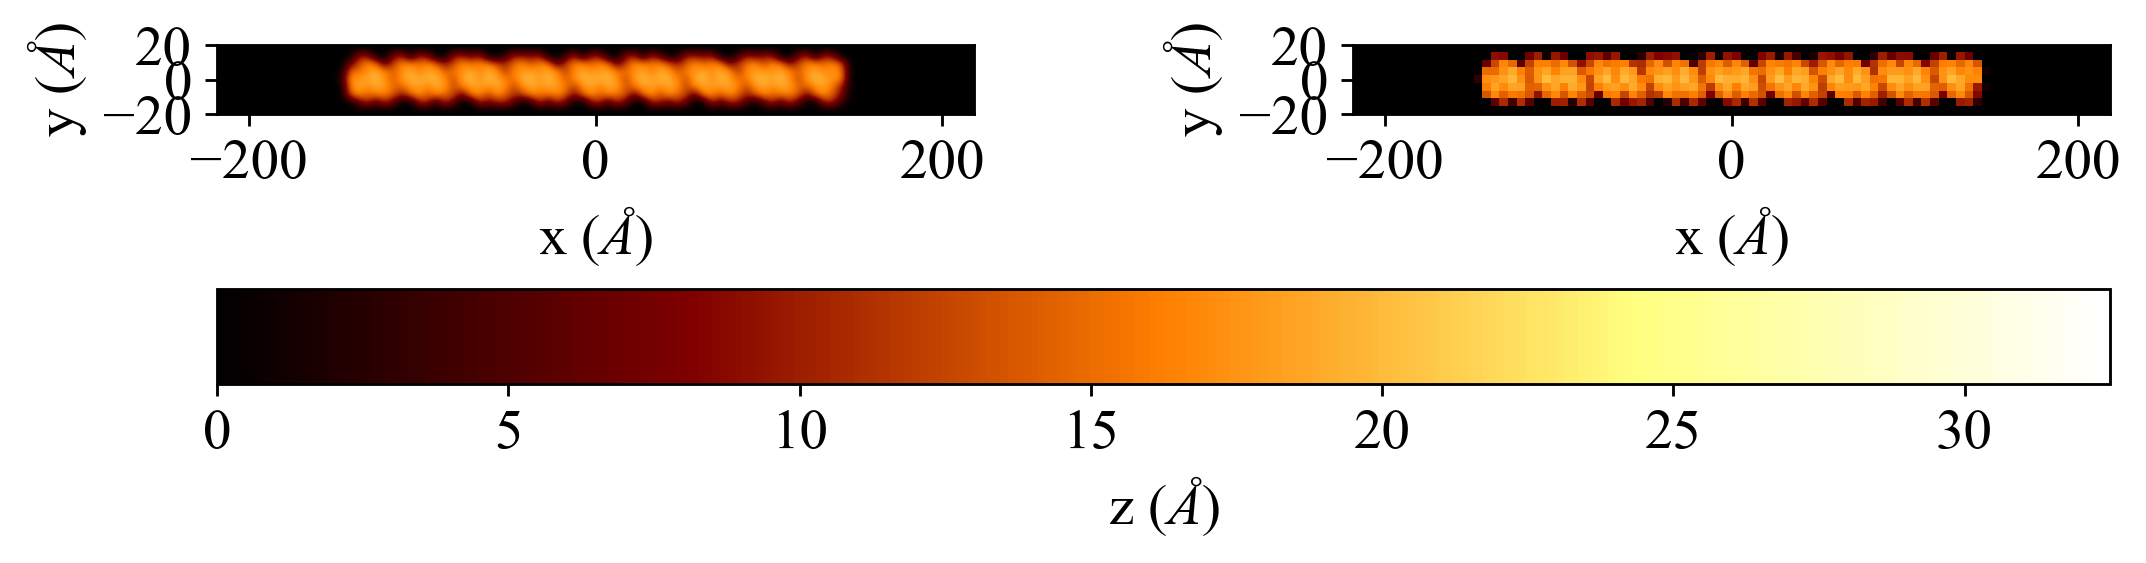
\includegraphics[width=1\linewidth]{Figures/AFMSimulationMolecule-bdna8_HS.png} 
    \end{subfigure}
    \hfill
    \begin{subfigure}[t]{1\textwidth}
        \centering
        \caption{\label{fig: PARP AFM Sim} }
        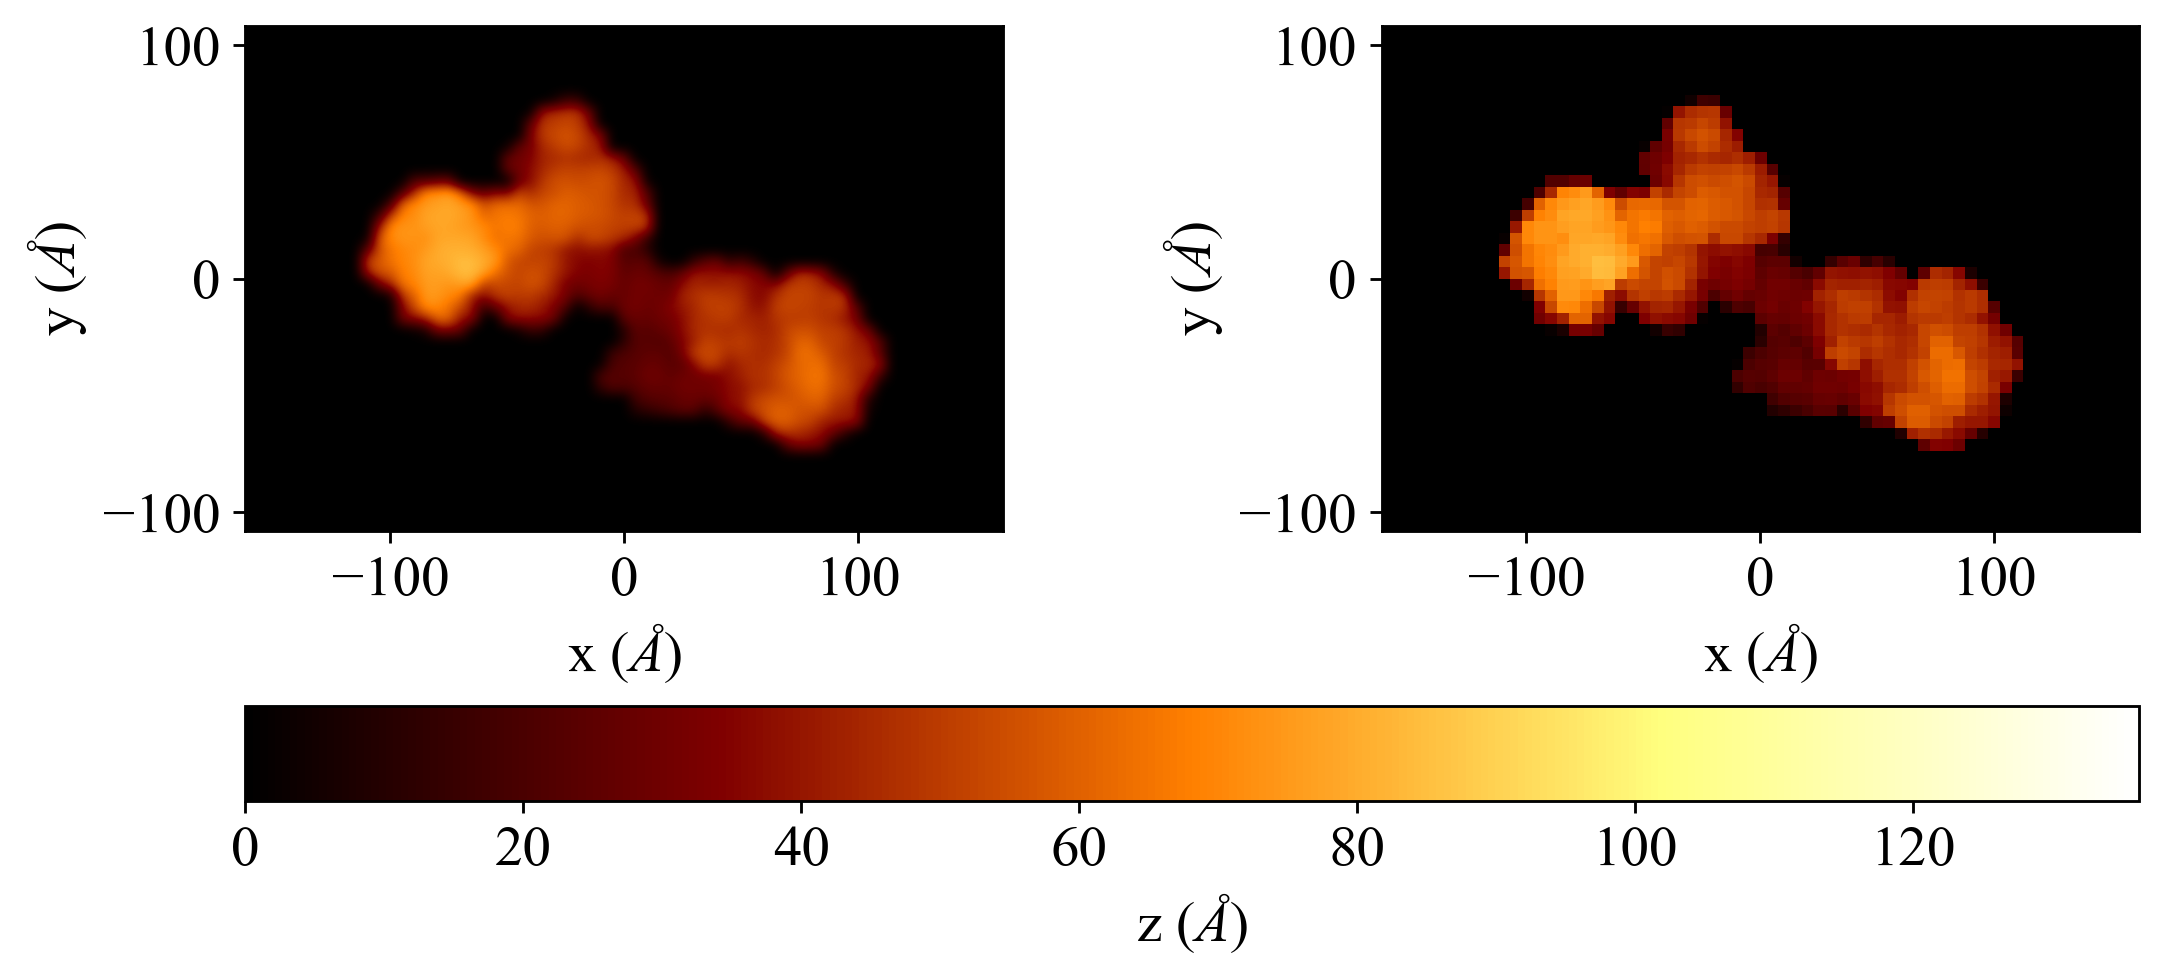
\includegraphics[width=1\linewidth]{Figures/AFMSimulationMolecule-4dqy_HS.png}
    \end{subfigure}
    \caption{\label{fig: AFM Simulation}Hard sphere model simulations of AFM image (A) DNA strand (custom pdb). (B) Human PARP-1 (PDB:4dqy).}
\end{figure}
